%20 min preso!
\documentclass[xcolor=table]{beamer}
\usepackage{beamerthemesplit}
\usepackage{wrapfig}
\usetheme{SPbGU}
\usepackage{pdfpages}
\usepackage{amsmath}
\usepackage{cmap}
\usepackage[T2A]{fontenc}
\usepackage[utf8]{inputenc}
\usepackage[english]{babel}
\usepackage{indentfirst}
\usepackage{amsmath}
\usepackage{tikz}
\usepackage{multirow}
\usepackage[noend]{algpseudocode}
\usepackage{algorithm}
\usepackage{algorithmicx}
\usepackage{fancyvrb}
\usetikzlibrary{calc}
\usetikzlibrary{shapes,arrows}
\usetikzlibrary{arrows,automata}
\usetikzlibrary{positioning}

\usepackage{tabularx}
\newcolumntype{Y}{>{\raggedleft\arraybackslash}X}

\renewcommand{\thealgorithm}{}

\newtheorem{mytheorem}{Theorem}
\renewcommand{\thealgorithm}{}

\newcommand{\tikzmark}[1]{\tikz[overlay,remember picture] \node (#1) {};}
\def\Put(#1,#2)#3{\leavevmode\makebox(0,0){\put(#1,#2){#3}}}

\newcommand{\ltz}{$< 1$}


\tikzset{
    state/.style={
           rectangle,
           rounded corners,
           draw=black, very thick,
           minimum height=2em,
           inner sep=2pt,
           text centered,
           },
}

\beamertemplatenavigationsymbolsempty

\title[CFPQ on GPGPU]{Evaluation of the Context-Free Path Querying Algorithm Based on Matrix Multiplication}
%\subtitle[YaccConstructor]{Parsing techniques for graph analysis}
% То, что в квадратных скобках, отображается в левом нижнем углу.
\institute[JetBrains Research]{
JetBrains Research, Programming Languages and Tools Lab  \\
Saint Petersburg University
}

% То, что в квадратных скобках, отображается в левом нижнем углу.
\author[Semyon Grigorev]{Nikita Mishin, Iaroslav Sokolov, Egor Spirin, Vladimir Kutuev, Egor Nemchinov, Sergey Gorbatyuk, \textbf{Semyon Grigorev}}

\date{June 30, 2019}

\begin{document}
{
\begin{frame}[fragile]
  \begin{table}
  \centering
  \begin{tabularx}{\linewidth}{YcX}
    
\includegraphics[height=1.5cm]{pictures/jetbrainsResearch.pdf} \hfill
    & \begin{minipage}[t]{0.3\textwidth}\center \vspace{-1cm}  GRADES-NDA 2019
      \end{minipage}
    & \hfill 
\includegraphics[height=1.5cm]{pictures/SPbGU_Logo.png}
  \end{tabularx}
  \end{table}
  \titlepage
\end{frame}
}

\begin{frame} \frametitle{Context-Free Path Querying}
  \begin{minipage}[m]{0.45\linewidth}
  \raisebox{-0.5\totalheight}{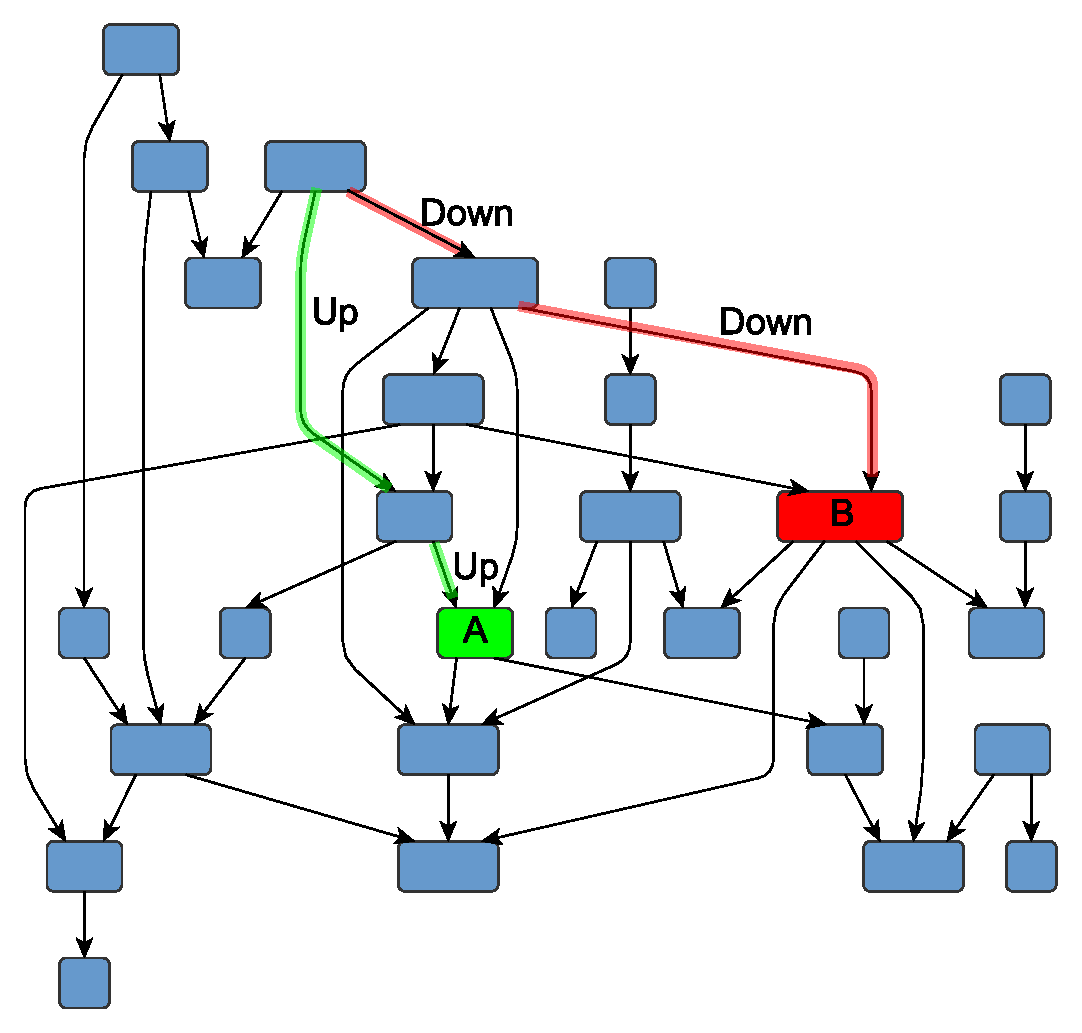
\includegraphics[width=\textwidth]{pictures/hierarchical.pdf}}
  \end{minipage}\hfill
  \begin{minipage}[m]{0.5\linewidth}
  Navigation through a graph
  \begin{itemize}
        \item Are nodes A and B on the same level of hierarchy?
        \item Is there a path of form $\textbf{Up}^n \, \textbf{Down}^n$?
        \item Find all paths of form $\textbf{Up}^n \, \textbf{Down}^n$ which start from the~node A
  \end{itemize}

  \end{minipage}

  \end{frame}

%  \begin{frame}[fragile] \frametitle{Applicatipons}
%    \begin{itemize}
%      \item Static code analysis
%      \item Graph database querying
%      \item RDF analysis
%    \end{itemize}
%  \end{frame}

  \begin{frame}[fragile]
    \frametitle{Context-Free Path Querying: Relational Query Semantics}
    \begin{itemize}
      \item $\mathbb{G} = (\Sigma, N, P)$ --- context-free grammar in normal form
      \begin{itemize}
        \item $A \rightarrow B C$, where $A, B, C \in N$
        \item $A \rightarrow x$, where $A \in N, x \in \Sigma$
        \item $L(\mathbb{G},A) = \{ \omega \mid A \rightarrow^* \omega \}$
      \end{itemize}
      \item $G = (V,E,L)$ --- directed graph
        \begin{itemize}
          \item $v \xrightarrow{l} u \in E$
          \item $L \subseteq \Sigma$
        \end{itemize}
      %\item $p = v_0 \xrightarrow{l_0} v_1 \xrightarrow{l_1} \cdots \xrightarrow{l_{n-2}} v_{n-1} \xrightarrow{l_{n-1}} v_n$ --- path in $G$
      \item $\omega(\pi) = \omega(v_0 \xrightarrow{l_0} v_1 \xrightarrow{l_1} \cdots \xrightarrow{l_{n-2}} v_{n-1} \xrightarrow{l_{n-1}} v_n) = l_0 l_1 \cdots l_{n-1}$
      \item $R_A = \{ (n, m) \mid \exists n \pi m$, such that $\omega(\pi) \in L(\mathbb{G},A)\}$
    \end{itemize}
  \end{frame}

  \begin{frame}[fragile] \frametitle{Matrix-Based Algorithm}
    \begin{algorithm}[H]
    \begin{algorithmic}[1]
    \caption{Context-Free Path Querying by Matrix Multiplication}
    \Function{contextFreePathQuerying}{D, G}

        \State{$n \gets$ the number of nodes in $D$}
        \State{$E \gets$ the directed edge-relation from $D$}
        \State{$P \gets$ the set of production rules in $G$}
        \State{$T \gets$ the matrix $n \times n$ in which each element is $\varnothing$}
        \ForAll{$(i,x,j) \in E$}
        \Comment{Matrix initialization}
            \State{$T_{i,j} \gets T_{i,j} \cup \{A~|~(A \rightarrow x) \in P \}$}
        \EndFor
        \While{matrix $T$ is changing}
            \State{$T \gets T \cup (T \times T)$}
            \Comment{Transitive closure $T^{cf}$ calculation}
        \EndWhile
    \State \Return $T$
    \EndFunction
    \end{algorithmic}
    \end{algorithm}
  \end{frame}


  \begin{frame}[fragile] \frametitle{Matrix-Based Algorithm: Technical Details}
    \begin{itemize}
      \item $T$ can be represented as e set of Boolean matrices: one matrix for each nonterminal
      \item The algorithm can be implemented in terms of Boolean matrices multiplication
      \item All matrices can be allocated in memory statically
    \end{itemize}
  \end{frame}


\begin{frame}[fragile] \frametitle{Research Questions}
  \begin{itemize}
    \item Can GPGPUs utilization for CFPQ improve performance in comparison with the CPU version?
    \pause
    \item Is it possible to achieve higher performance by means of existing libraries for matrices operations or do we need to create our own solution to get more control?
    \pause
    \item Can we achieve high performance with high-level languages such as Python?
    \pause
    \item Can we improve performance by using sparse matrix representation for CFPQ?
  \end{itemize}
\end{frame}


\begin{frame}[fragile] \frametitle{CPU-Based Implementations}
  \begin{minipage}[t]{1cm}
\hspace{1cm}
  \end{minipage}
  ~
\begin{minipage}[t]{0.85\textwidth}
\begin{itemize}
  \item[\textbf{[Scipy]}] Sparse matrices multiplication by using \textbf{Scipy} in \textbf{Python} programming language
\pause
  \item[\textbf{[M4RI]}] Dense matrices multiplication by using \textbf{m4ri2} library which implements the Method of Four Russians in \textbf{C} language
\end{itemize}
\end{minipage}
\end{frame}


\begin{frame}[fragile] \frametitle{GPGPU-Based Implementations}
  \begin{minipage}[t]{1cm}
\hspace{1cm}
  \end{minipage}
  ~
\begin{minipage}[t]{0.85\textwidth}
\begin{itemize}
\item[\textbf{[GPU4R]}] Our own implementation of the Method of Four
Russians in \textbf{CUDA C}
\pause
\item[\textbf{[GPU\_N]}] Our own implementation of the na\"{\i}ve boolean
matrix multiplication in \textbf{CUDA C}
\pause
\item[\textbf{[GPU\_Py]}] Manual implementation of na\"{\i}ve boolean matrix
multiplication in \textbf{Python} by using \textbf{numba} compiler
\end{itemize}
\end{minipage}
\end{frame}

\begin{frame}[fragile] \frametitle{Reference Implementations}
  \begin{minipage}[t]{1cm}
\hspace{1cm}
  \end{minipage}
  ~
\begin{minipage}[t]{0.85\textwidth}
\begin{itemize}
\item[\textbf{[CuSprs]}]
\begin{itemize}
  \item Rustam Azimov, 2018, ``Context-free Path Querying by Matrix Multiplication''
  \item Implementation is based on NVIDIA cuSPARSE library (\textbf{CUDA C, GPGPU})
\end{itemize}
\pause
\item[\textbf{[CYK]}]
\begin{itemize}
  \item X. Zhang et al, 2016, ``Context-free path queries on RDF graphs''
  \item CYK-based algorithm implemented in \textbf{Java} (CPU)
\end{itemize}
\end{itemize}
\end{minipage}
\end{frame}


\begin{frame}[fragile] \frametitle{Dataset}
  \begin{minipage}[t]{1cm}
\hspace{1cm}
  \end{minipage}
  ~
\begin{minipage}[t]{0.85\textwidth}
\begin{itemize}
\item[\textbf{[RDF]}]
\begin{itemize}
  \item The set of the real-world RDF files (ontologies)
  \item Queries: $G_4: s \to SCOR \ s \ SCO \ | \ TR \ s \ T \ | \ SCOR \ SCO \ | \ TR \ T$,
$G_5: s \to SCOR \ s \ SCO \ | \ SCO$
\end{itemize}

\pause
\item[\textbf{[Worst]}]
\begin{itemize}
  \item The input graph is a two cycles of coprime lengths with a single common vertex
  \begin{figure}
        \begin{tikzpicture}[shorten >=1pt,node distance=2cm,on grid,auto]
   \node[state] (q_1)   {$1$};
   \node[state] (q_2) [above=of q_1] {$2$};
   \node[state] (q_3) [above right=of q_1, below right=of q_2] {$0$};
   \node[state] (q_4) [right=of q_3] {$3$};
    \path[->]
    (q_1) edge  node {A} (q_2)
    (q_2) edge  node {A} (q_3)
    (q_3) edge  node {A} (q_1)
    (q_3) edge[bend left, above]  node {B} (q_4)
    (q_4) edge[bend left, below]  node {B} (q_3);
\end{tikzpicture}
\end{figure}
  \item Queries: $G_1: s \to A \ s \ B \ | \ A \ B$
\end{itemize}
\end{itemize}
\end{minipage}
\end{frame}

\begin{frame}[fragile] \frametitle{Dataset}
  \begin{minipage}[t]{1cm}
\hspace{1cm}
  \end{minipage}
  ~
\begin{minipage}[t]{0.85\textwidth}
\begin{itemize}
\item[\textbf{[Full]}]
\begin{itemize}
  \item The input graph is sparse, but the result is a full graph
  \item Queries: \\ $G_2: s \to s \ s \ | \ A$, \\ $G_3: s \to s \ s \ s \ | \ A$
\end{itemize}
\pause
\item[\textbf{[Sparse]}]
\begin{itemize}
  \item Sparse graphs are generated by the GTgraph
  \item Queries: $G_1: s \to A \ s \ B \ | \ A \ B$
\end{itemize}
\end{itemize}
\end{minipage}
\end{frame}

\begin{frame} \frametitle{Evaluation}
  \begin{itemize}
   \item OS: Ubuntu 18.04
   \item CPU: Intel core i7 8700k 3,7HGz
   \item RAM: DDR4 32 Gb
   \item GPGPU: Geforce 1080Ti (11Gb RAM)
  \end{itemize}
\end{frame}

\begin{frame}[fragile] \frametitle{Evaluation: [RDF]\footnote{Time in milliseconds}}
\begin{center}
  {\tiny
  \rowcolors{1}{}{lightgray}
  \begin{tabular}{| p{1.25cm} | c | c | c | c | c | c | c | c | c |}
      \hline
      \multicolumn{3}{|c|}{RDF}        & \multicolumn{7}{|c|}{Query $G_4$}  \\
      \hline
      Name                                & \#V & \#E  & Scipy & M4RI  & GPU4R & GPU\_N & GPU\_Py & CuSprs & CYK~\footnote{Results from X. Zhang et al, 2016, ``Context-Free Path Queries on RDF Graphs''} \\
      \hline
      \hline
      \tiny{atm-prim}                    & 291 & 685  & 3     &  2    & 2     & 1      & 5       & 269  & 515285  \\
      \tiny{biomed}                      & 341 & 711  & 3     &  5    & 2     & 1      & 5       & 283  & 420604  \\
      \tiny{foaf}                        & 256 & 815  & 2     &  9    & 2     & \ltz   & 5       & 270  & 5027    \\
      \tiny{funding}                     & 778 & 1480 & 4     &  7    & 4     & 1      & 5       & 279  & 499     \\
      \tiny{generations}                 & 129 & 351  & 3     &  3    & 2     & \ltz   & 5       & 273  & 6091    \\
      \tiny{people\_pets}                & 337 & 834  & 3     &  3    & 3     & 1      & 7       & 284  & 82081   \\
      \tiny{pizza}                       & 671 & 2604 & 6     &  8    & 3     & 1      & 6       & 292  & 3233587 \\
      \tiny{skos}                        & 144 & 323  & 2     &  4    & 2     & \ltz   & 5       & 273  & 1044    \\
      \tiny{travel}                      & 131 & 397  & 3     &  5    & 2     & \ltz   & 6       & 268  & 13971   \\
      \tiny{unv-bnch}                    & 179 & 413  & 2     &  4    & 2     & \ltz   & 5       & 266  & 20981   \\
      \tiny{wine}                        & 733 & 2450 & 7     &  6    & 4     & 1      & 7       & 294  & 4075319 \\
      \hline
    \end{tabular}
    }
  %  {\tiny
  %    \rowcolors{1}{}{lightgray}
  %    \begin{tabular}{| p{1.25cm} | c | c | c | c | c | c | c | c | }
  %        \hline
  %        \multicolumn{3}{|c|}{RDF}        & \multicolumn{6}{|c|}{Query %$G_5$}                              \\
  %        %\cline{2-13}
  %        \hline
  %        Name                                & \#V & \#E  & Scipy & M4RI  & GPU4R & GPU\_N & GPU\_Py & %CuSprs \\
  %        \hline
  %        \hline
  %        \tiny{atm-prim}                    & 291 & 685   & 1     & \ltz & 1     & \ltz   & 2       & %267  \\
  %        \tiny{biomed}                      & 341 & 711   & 4     & \ltz & 1     & \ltz   & 5       & %280  \\
  %        \tiny{foaf}                        & 256 & 815   & 1     & \ltz & 1     & \ltz   & 2       & %263  \\
  %        \tiny{funding}                     & 778 & 1480  & 2     & \ltz & 3     & \ltz   & 4       & %274  \\
  %        \tiny{generations}                 & 129 & 351   & 1     & \ltz & 1     & \ltz   & 2       & %263  \\
  %        \tiny{people\_pets}                & 337 & 834   & 1     & \ltz & 1     & \ltz   & 3       & %277  \\
  %        \tiny{pizza}                       & 671 & 2604  & 2     & \ltz & 2     & \ltz   & 5       & %278  \\
  %        \tiny{skos}                        & 144 & 323   & \ltz  & \ltz & 1     & \ltz   & 2       & %265  \\
  %        \tiny{travel}                      & 131 & 397   & 1     & \ltz & 1     & \ltz   & 3       & %271  \\
  %        \tiny{unv-bnch}                    & 179 & 413   & 1     & \ltz & 1     & \ltz   & 3       & %266  \\
  %        \tiny{wine}                        & 733 & 2450  & 1     & \ltz & 3     & \ltz   & 3       & %281  \\
  %        \hline
  %      \end{tabular}
  %      }
        \end{center}

\end{frame}


\begin{frame} \frametitle{Evaluation: [Worst]\footnote{Time in seconds}}
  \begin{centering}
  \rowcolors{1}{}{lightgray}
  \begin{tabular}{| l | c | c | c | c | c | c | }
      \hline
      \#V  & Scipy    & M4RI    & GPU4R  & GPU\_N  & GPU\_Py & CuSprs   \\
      \hline
      \hline
      16   & 0.032    & $< 0.001$    & 0.008  & 0.002   & 0.027   & 0.309    \\
      32   & 0.118    & 0.001   & 0.034  & 0.008   & 0.136   & 0.441    \\
      64   & 0.476    & 0.041   & 0.133  & 0.032   & 0.524   & 0.988    \\
      128  & 2.194    & 0.226   & 0.562  & 0.129   & 2.751   & 3.470    \\
      256  & 15.299   & 1.994   & 3.088  & 0.544   & 11.883  & 15.317   \\
      512  & 121.287  & 23.204  & 13.685 & 2.499   & 43.563  & 102.269  \\
      1024 & 1593.284 & 528.521 & 88.064 & 19.357  & 217.326 & 1122.055 \\
      2048 & -        & -       & -      & 325.174 & -       & -        \\
      \hline
    \end{tabular}
  \end{centering}
\end{frame}

\begin{frame} \frametitle{Evaluation: [Sparse]\footnote{Time in seconds}}

{\small
  \rowcolors{1}{}{lightgray}
  \begin{tabular}{| l | c | c | c | c | c | c | }
      \hline
      Graph              & Scipy   & M4RI     & GPU4R  & GPU\_N & GPU\_Py & CuSprs  \\
      \hline
      \hline
      \small{G5k-0.001}  & 10.352  & 0.647    & 0.113  & 0.041  & 0.216   & 5.729   \\
      \small{G10k-0.001} & 37.286  & 2.395    & 0.435  & 0.215  & 1.331   & 35.937  \\
      \small{G10k-0.01}  & 97.607  & 1.455    & 0.273  & 0.138  & 0.763   & 47.525  \\
      \small{G10k-0.1}   & 601.182 & 1.050    & 0.223  & 0.114  & 0.859   & 395.393 \\
      \small{G20k-0.001} & 150.774 & 11.025   & 1.842  & 1.274  & 6.180   & -       \\
      \small{G40k-0.001} & -       & 97.841   & 11.663 & 8.393  & 37.821  & -       \\
      \small{G80k-0.001} & -       & 1142.959 & 88.366 & 65.886 & -       & -       \\
      \hline
    \end{tabular}
}
\end{frame}


\begin{frame}[fragile] \frametitle{Evaluation: [Full]\footnote{Time in seconds}}
\begin{center}
  {\small
  \rowcolors{1}{}{lightgray}
  \begin{tabular}{| l | c | c | c | c | c | c |}
      \hline
      \multirow{2}{*}{\#V} & \multicolumn{6}{|c|}{Query $G_2$}  \\
      \cline{2-7}
                           & Scipy   & M4RI    & GPU4R   & GPU\_N  & GPU\_Py & CuSprs  \\
      \hline
      \hline
      100                  & 0.007   & 0.002    & 0.002   & $< 0.001$    & 0.003   & 0.278       \\
      200                  & 0.040   & 0.003    & 0.002   & 0.001   & 0.004   & 0.279       \\
      500                  & 0.480   & 0.003    & 0.003   & 0.001   & 0.004   & 0.329       \\
      1000                 & 3.741   & 0.007    & 0.005   & 0.001   & 0.006   & 0.571       \\
      2000                 & 40.309  & 0.063    & 0.019   & 0.003   & 0.017   & 1.949       \\
      5000                 & 651.343 & 0.366    & 0.125   & 0.038   & 0.150   & 99.651      \\
      10000                & -       & 1.932    & 0.552   & 0.315   & 0.840   & 1029.042    \\
      25000                & -       & 33.236   & 7.252   & 5.314   & 15.521  & -           \\
      50000                & -       & 360.035  & 58.751  & 44.611  & 129.641 & -           \\
      80000                & -       & 1292.817 & 256.579 & 190.343 & 641.260 & -           \\

      \hline
    \end{tabular}
    }
    \end{center}
\end{frame}


\begin{frame}[fragile] \frametitle{Conclusion}
  \begin{itemize}
    \item GPGPUs utilization significantly increases the performance of CFPQ
    \pause
    \item High performnce libraries utilization is a good idea
    \begin{itemize}
      \item But it should be an appropriate libraries: M4RI (CPU) is better then cuSPARSE (GPGPU)
    \end{itemize}
    \pause
    \item High level languages + translator to GPGPU may be a good balance between performance ad implementation complexity
    \pause
    \item Sparse matrix representation is important for performance ([Scipy] for [Sparse])
    \begin{itemize}
      \item We should try to implement sparse boolean matrix operations for GPGPU
    \end{itemize}
  \end{itemize}
\end{frame}

\begin{frame}[fragile] \frametitle{Future Research}
  \begin{itemize}
    \item Detailed investigation of implemented algorithms
    \item Create open extensible platform for CFPQ algorithms comparison
    \item Evaluate other CFPQ algorithms
    \begin{itemize}
      \item Sparse matrices
      \item Destributed matrix multiplication
      \item LL and LR parsing algorithms
    \end{itemize}
    \item Add new data and queries
    \begin{itemize}
      \item Big RDFs
      \item Static code analysis
    \end{itemize}
  \end{itemize}
\end{frame}

\begin{frame}
\frametitle{Contact Information}
\begin{itemize}
  \item Semyon Grigorev:
    \begin{itemize}
      \item \href{mailto:s.v.grigoriev@spbu.ru}{s.v.grigoriev@spbu.ru}
      \item \href{mailto:Semen.Grigorev@jetbrains.com}{Semen.Grigorev@jetbrains.com}
    \end{itemize}
  \item Nikita Mishin: \href{mailto:mishinnikitam@gmail.com}{mishinnikitam@gmail.com}
  \item Iaroslav Sokolov: \href{mailto:sokolov.yas@gmail.com}{sokolov.yas@gmail.com}
  \item Egor Spirin: \href{mailto:egor@spirin.tech}{egor@spirin.tech}
  \item Vladimir Kutuev: \href{mailto:vladimir.kutuev@gmail.com}{vladimir.kutuev@gmail.com}
  \item Egor Nemchinov: \href{mailto:nemchegor@gmail.com}{nemchegor@gmail.com}
  \item Sergey Gorbatyuk: \href{mailto:sergeygorbatyuk171@gmail.com}{sergeygorbatyuk171@gmail.com}
\vspace{0.5cm}
  \item Dataset and algorithm implementations: \href{https://github.com/SokolovYaroslav/CFPQ-on-GPGPU}{https://github.com/SokolovYaroslav/CFPQ-on-GPGPU}
\end{itemize}
\vspace{0.1cm}
\center{\huge{Thanks!}}
\end{frame}
\end{document}
